%!TEX TS-program = xelatex
%!TEX encoding = UTF-8 Unicode



Basandonos en el algoritmo de Louvain para la conformacion de clusters es que comenzamos el analisis para cada estadio del sueño (W, N1, N2 y N3) y se calculó el promedio de las matrices de adyacencia de los 18 sujetos informados en el dataset.
Utilizando las distintas densidades de aristas fuimos creando grafos no pesados, para luego aplicar el algoritmo de clustering.

Para estudiar los resultados, se eligieron dos medidas de clustering \textbf{el coeficiente de modularidad y el número
de comunidades o módulos encontrados}


\begin{figure}[H]
    \centering
    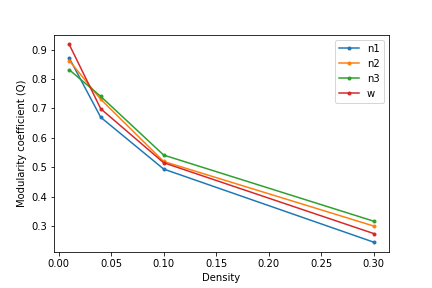
\includegraphics[width=\textwidth]{img/2_mod_coeff.png}
    \caption{Coeficiente de modularidad (Q) en función de las densidades}
    \label{fig:2_mod_coeff}
\end{figure}

Se observa que \textbf{Q} se decrementa en todos los casos a medida que la \textbf{densidad} aumenta. A partir de una \textbf{densidad = 0.15} la tendencia evidencia que los estadios se comportan asintoticamente y con una tendencia a la baja siendo \textbf{n3 > n2 > w > n1}.


\begin{figure}[H]
    \centering
    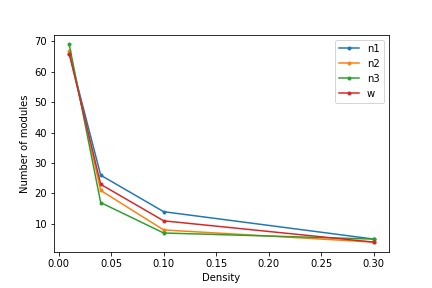
\includegraphics[width=\textwidth]{img/2_number_mod.png}
    \caption{Número de comunidades (Nc) en función de las densidades}
    \label{fig:2_number_mod}
\end{figure}

El numero de \textbf{comunidades} se decrementa fuertemente en el intervalo que va de 0 a 0.10 de la densidad. Luego siguen disminuyendo pero a una velocidad menor pero con una tendencia sostenida que permite afirmar que al igual que con el \textbf{Q}, a mayor \textbf{densidad} menor numero de \textbf{comunidades}.




\subsection{Redes Random}

Se vuelven a hacer los estudios anteriores pero esta vez comparando las distintas medidas de clustering contra una red random que preserva la distribución de grados de los nodos.


\begin{figure}[H]
    \centering
    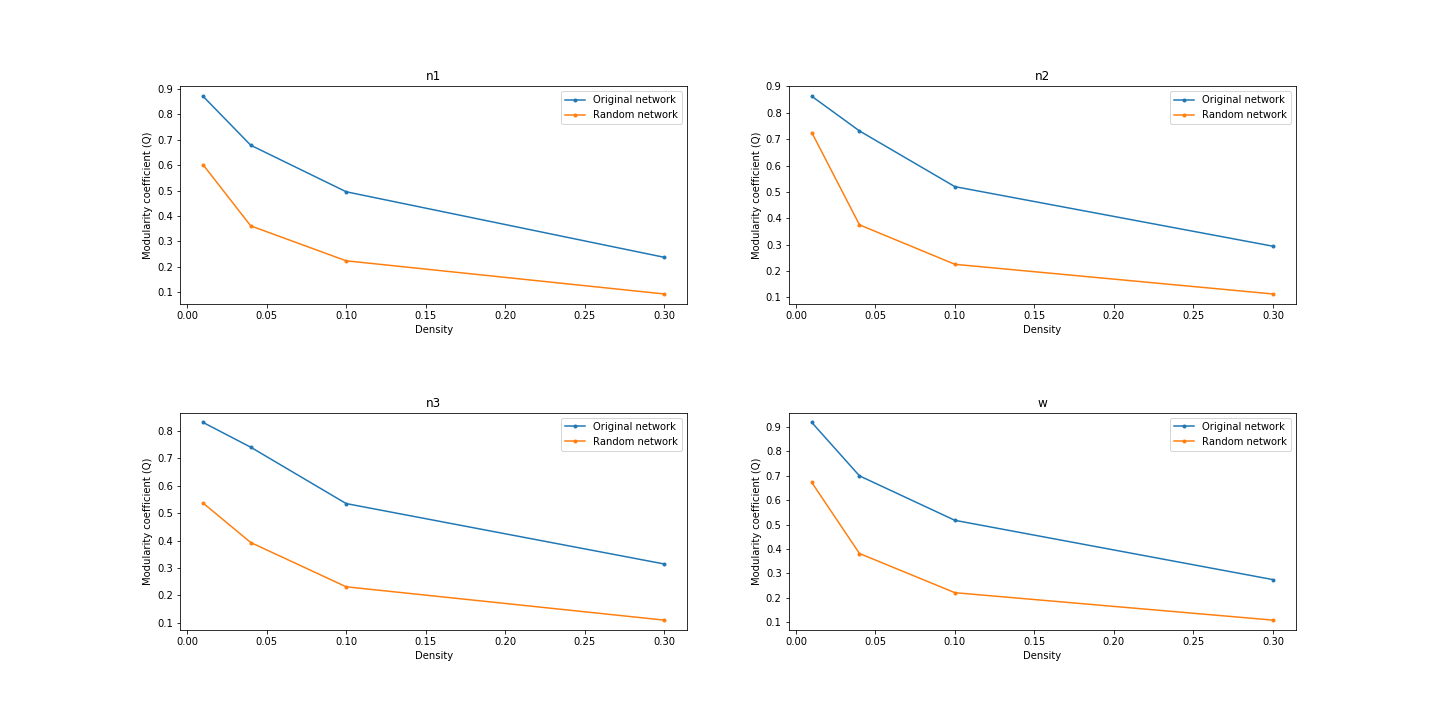
\includegraphics[width=\textwidth]{img/2_mod_coeff_vs_random.png}
    \caption{Red original vs Random - coeficiente de modularidad (Q) en función de las densidades}
    \label{fig:2_mod_coeff_vs_random}
\end{figure}

Al estudiar por separado los cuatro estadios del sueño y compara el \textbf{Q} tanto para la red original vs una red random, podemos observar que la red random muentra en todos los casos valores menores de \textbf{Q} para una densidad dada, pero conserva la misma tendencia de la red original de decrecer el \textbf{Q} a medida que aumenta la \textbf{densidad}




\begin{figure}[H]
    \centering
    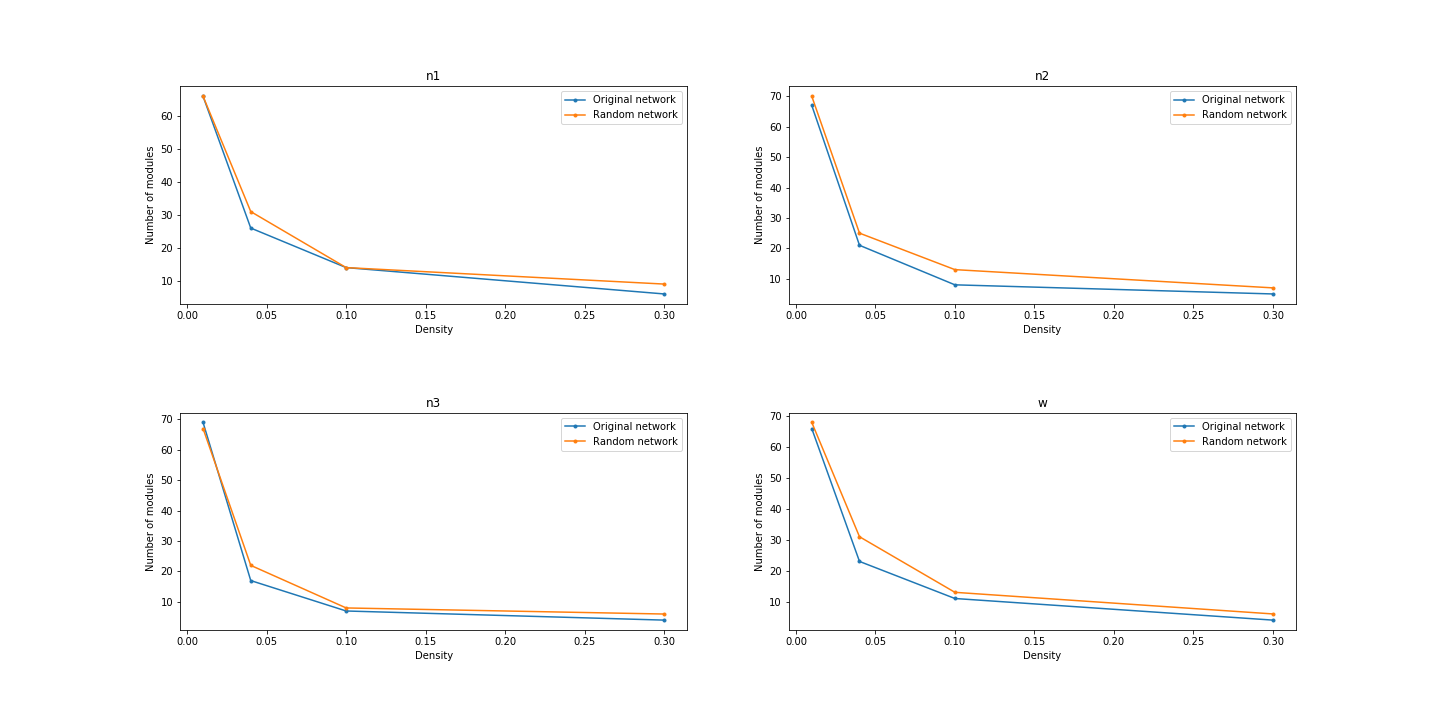
\includegraphics[width=\textwidth]{img/2_number_modules_vs_random.png}
    \caption{Red original vs Random - Número de comunidades (Nc) en función de las densidades}
    \label{fig:2_number_modules_vs_random}
\end{figure}


Para el caso de las \textbf{comunidades}, si bien la tendencia es la misma que la enunciada con anterioridad, en este caso la red random muesta valores de comunidades ligeramente mayores o iguales que la red original. Para el caso del estadio $n3$ y en especial el $n1$ las curvas se igualan en algunos puntos.